\section{Social Media - II Lecture}

Welcome to part two of our class on social media. In the previous
session, we discussed the concept of crowdsourcing and its application.
To illustrate this, we used the Nike example.

\subsection{Crowdsourcing and
    Co-Creation}\label{crowdsourcing-and-co-creation}

\subsubsection{Understanding Co-Creation}\label{understanding-co-creation}

\begin{figure}[!h]
    \centering
    \includegraphics[page=11, trim = 1.5cm 3cm 2.5cm 3cm, clip, width=\textwidth]{images/04 - Social_Media.pdf}
\end{figure}

Nike leverages the power of the crowd, which includes both potential and
existing customers, to gather feedback, generate ideas, and shape new
products and assortments. By utilizing crowdsourcing and co-creation,
Nike aims to collaborate with its customers in the innovation process.
Co-creation involves partnering with customers to define, create, and
develop new products or services. This approach aligns with the
principles of crowdsourcing discussed earlier.

Through co-creation, Nike gains valuable insights into sales priorities
for its assortment and identifies emerging trends for new products. This
innovative paradigm allows Nike to tap into the collective intelligence
and creativity of its customer base, resulting in a more
customer-centric approach to product development. By embracing
co-creation and crowdsourcing, Nike is able to stay at the forefront of
innovation in the industry.

\subsubsection{Direct vs Indirect
    Co-Creation}\label{direct-vs-indirect-co-creation}

In co-creation, the collaboration between a supplier and customers can
take two forms: direct or indirect. Direct co-creation occurs when
customers are aware that they are participating in an innovation process
and actively choose to contribute. They understand their role in the
process and willingly engage in it. On the other hand, indirect
co-creation happens when customers are unknowingly involved in the
innovation process. They may provide suggestions, comments, or opinions
without being prompted by the company. The company can listen to these
discussions on social media and use the inputs received to develop new
products or services, even if the customers are unaware that their
contributions are being utilized.

When companies are new to co-creation, they typically start with an
indirect approach. They listen to the open and spontaneous discussions
that customers have about their products and may gather feedback without
explicitly informing customers that they are participating in a
co-creation initiative. This initial step allows companies to understand
customer perspectives. Once they have gained experience and confidence,
companies can then move on to direct co-creation initiatives that
explicitly require the deliberate participation of customers.

\subsubsection{The Importance of
    Listening}\label{the-importance-of-listening}

\begin{figure}[!h]
    \centering
    \includegraphics[page=12, trim = 1.5cm 7cm 2.5cm 4cm, clip, width=\textwidth]{images/04 - Social_Media.pdf}
\end{figure}

The importance of listening before engaging in direct co-creation lies
in understanding what customers already think about your products. By
starting with listening, you can gather valuable feedback that will
guide the direction of your co-creation initiatives. Launching a
co-creation project without prior knowledge of customer feedback may
result in having to align your efforts with their expectations.
Therefore, it is more beneficial to proactively seek out and analyze the
spontaneous feedback customers provide on social media. This listening
process not only helps in shaping co-creation initiatives but also
provides valuable insights for product and service innovation.

\subsubsection{Transitioning to Direct
    Co-Creation}\label{transitioning-to-direct-co-creation}

\begin{figure}[!h]
    \centering
    \includegraphics[page=13, trim = 1cm 6cm 3cm 4cm, clip, width=\textwidth]{images/04 - Social_Media.pdf}
\end{figure}

In simpler terms, companies can benefit from the comments and feedback
that customers provide voluntarily and for free. This information can be
used to design new products and services or improve existing ones
without explicitly launching a co-creation initiative. Once the company
is ready, they can then transition to direct co-creation.

\subsection{Expanding the Scope of
    Co-Creation}\label{expanding-the-scope-of-co-creation}

\subsubsection{Beyond Private
    Communities}\label{beyond-private-communities}

Now, let's talk about indirect co-creation. To expand the scope of
co-creation, it's important to listen not only to the community within
the company's private label community but also to the wider community
outside of it. Let's use Vodafone as an example. Vodafone has its own
private social platform called Vodafone Lab, where they listen to what
their customers have to say. However, this platform is limited to
customers who are already positive about Vodafone and remain loyal to
the brand. As a result, the feedback they receive may not include the
main reasons why other customers choose to leave Vodafone or why they
choose a different provider. Therefore, it's crucial to have a
360-degree approach to listening, not just limited to your own clients.
Companies often focus solely on their existing customer base, but this
can be a limitation when it comes to gathering valuable insights.

\subsubsection{Leveraging Influencers}\label{leveraging-influencers}

To launch successful co-creation initiatives, companies need to address
the challenge of motivating people to participate. Crowdsourcing, which
is the basis of co-creation, relies on the crowd performing tasks that
require time and effort. However, simply relying on the company's brand
or reputation may not be enough to attract participants. This is where
leveraging influencers becomes crucial.

Companies can identify influencers in the industries they operate in and
collaborate with them to drive co-creation. Influencers, who are opinion
leaders in their respective fields, have a strong presence on social
media and can help generate interest and engagement. The advantage of
working with influencers is that they are motivated by financial
incentives. By compensating them for their contributions, companies can
ensure their active participation in co-creation initiatives.

Paying influencers not only guarantees their involvement but also allows
companies to tap into their expertise and leadership within their
tribes. This approach provides a win-win situation: influencers monetize
their position and companies benefit from their valuable insights.
Additionally, influencers will share their opinions on social media,
further amplifying the reach and impact of the co-creation initiative.

\subsubsection{Designing Effective Co-Creation
    Initiatives}\label{designing-effective-co-creation-initiatives}

\begin{figure}[!h]
    \centering
    \includegraphics[page=15, trim = 1.5cm 6cm 3cm 4cm, clip, width=\textwidth]{images/04 - Social_Media.pdf}
\end{figure}

In addition to running co-creation initiatives limited to influencers,
companies can also make an effort to involve their entire customer base.
The goal is to engage influencers, compensate them for their
participation, and rely on them to spread the co-created products to a
wider audience. Paying influencers to promote the products increases the
chances of influencing the crowd, as there have been many success
stories in this regard.

\begin{figure}[!h]
    \centering
    \includegraphics[page=16, trim = 0cm 5cm 3cm 5cm, clip, width=\textwidth]{images/04 - Social_Media.pdf}
\end{figure}

However, the main risk of expanding co-creation initiatives beyond
influencers and involving direct client participation is the lack of
effective encouragement and coordination of contributions. There is a
possibility that clients may not contribute as expected, resulting in a
failed initiative. To mitigate this risk, there is a checklist of design
variables for co-creation initiatives. This includes determining the
participation mechanisms, selecting the appropriate technology platform,
defining precise roles and tasks for community members, identifying the
types of users to involve, establishing an incentive system to motivate
participation, and implementing quality control mechanisms to ensure
high-quality content.

Co-creation initiatives are like creating a small social network, and it
is crucial to prioritize the quality of content. The content itself is
more important than the content creator. Therefore, low-quality content
should be discarded, and the co-creation initiatives should be properly
moderated and coordinated.

\subsection{Marketing and Communication
    Strategies}\label{marketing-and-communication-strategies}

\subsubsection{Traditional Marketing and
    Broadcasting}\label{traditional-marketing-and-broadcasting}

\begin{figure}[!h]
    \centering
    \includegraphics[page=17, trim = 1.5cm 5cm 2.5cm 3cm, clip, width=\textwidth]{images/04 - Social_Media.pdf}
\end{figure}

The checklist provided here goes beyond the traditional knowledge that
marketers typically possess. Marketing is often defined as having a
marketing orientation, which means understanding and responding to
existing market needs. However, throughout history, companies have also
been able to influence the market by investing in marketing initiatives.
By allocating sufficient resources, companies can create a demand for a
new product or service that may not have existed before. For example, a
fashion designer with a new idea must create awareness and generate
interest in their product through marketing efforts. Marketing is not
just about responding to existing needs; it's also about sensing a need,
creating awareness for that need, and then responding to it. In essence,
marketing involves both sensing and driving the market.

Traditionally, companies have used broadcasting as a means to achieve
this. Broadcasting refers to the company speaking through a channel that
reaches a wide audience simultaneously, such as television. For
instance, a company designs an advertisement and broadcasts it on TV
during prime time, when the audience is at its broadest. The audience
receives the content but does not have the opportunity to respond
directly. This form of communication is one-way, with the company
broadcasting its message to potential clients.

\subsubsection{Social Media
    Communication}\label{social-media-communication}

\begin{figure}[!h]
    \centering
    \includegraphics[page=18, trim = 1.5cm 4.5cm 3cm 0.5cm, clip, width=\textwidth]{images/04 - Social_Media.pdf}
\end{figure}

There is a distinct difference between
broadcasting and social media communication. Unlike broadcasting, where
only the broadcaster has the opportunity to speak, social media allows
both the audience and the broadcaster to engage in conversation. While
they may speak at different times, it is essential that both parties
have the chance to express themselves.

Social media platforms serve as communication channels, enabling the
audience to actively participate. Users can respond to content and leave
comments, fostering a two-way interaction. In the field of marketing,
there is a well-known distinction between ``above the line'' and ``below
the line'' strategies. ``Above the line'' refers to broadcasting, while
``below the line'' encompasses social media communication channels.

\subsubsection{Viral Marketing and
    Influencers}\label{viral-marketing-and-influencers}

\begin{figure}[!h]
    \centering
    \includegraphics[page=19, trim = 2cm 7cm 3cm 4cm, clip, width=\textwidth]{images/04 - Social_Media.pdf}
\end{figure}

In marketing, there is a clear distinction between below
the line and above the line strategies. When something is successful on
social media, it can easily be broadcasted to a wider audience. However,
the reverse is not true. Content that performs well on traditional
broadcasting channels may not be suitable for social media, as it can
attract negative comments from a vocal minority. These negative comments
can have a detrimental effect on the brand and its reputation among the
broader social audience.

On social media, there is a group of individuals known as ``haters'' who
are particularly aggressive and negative in their comments. Their
opinions can influence the perception of the broader audience, and there
is no way to control or govern what they say. To counteract this, it is
important to activate viral marketing on social media. This involves
creating high-quality content that is suitable for the platform and does
not incite hate or offense. While the reach of an influencer with
100,000 followers may not compare to a prime-time broadcasting channel
with millions of viewers, viral marketing has the potential to reach
hundreds of millions of users on social media.

\begin{figure}[!h]
    \centering
    \includegraphics[page=20, trim = 1cm 0cm 2cm 1cm, clip, width=\textwidth]{images/04 - Social_Media.pdf}
\end{figure}

However, it is important to note that people have the freedom to choose
whether or not to share content. To encourage sharing, the content needs
to be viral and capable of generating word-of-mouth. This is where
influencers play a powerful role. As tribe leaders, influencers have a
loyal following who are more likely to share their content simply
because it comes from someone they admire and trust.

\subsection{Governance and Process in Social
    Media}\label{governance-and-process-in-social-media}

\subsubsection{The Virality and Volatility of Social
    Media}\label{the-virality-and-volatility-of-social-media}

\begin{figure}[!h]
    \centering
    \includegraphics[page=21, trim = 2cm 8cm 3cm 4cm, clip, width=\textwidth]{images/04 - Social_Media.pdf}
\end{figure}

\begin{figure}[!h]
    \centering
    \includegraphics[page=22, trim = 2cm 5cm 3cm 3.5cm, clip, width=\textwidth]{images/04 - Social_Media.pdf}
\end{figure}

On social media, attention is fleeting and trends come and go in an
instant. The pace is incredibly fast, with a massive influx of posts
that quickly fade into obscurity. Take a look at this list of global
fashion influencers. You'll recognize some familiar names. To succeed on
social media, you need to continuously generate buzz and keep the
word-of-mouth going. It requires endurance and stamina to consistently
produce engaging content in the hopes of it going viral. Interestingly,
negative news tends to attract more attention than positive news in
traditional media. The question is, does the same hold true for social
media? The answer is yes. Even on social media, negative content tends
to be retweeted more than positive feedback and posts. This is why
haters often take the easy route. However, it's important to note that
tweets have a short lifespan, with 80 percent of retweets occurring
within the first 30 minutes of posting. Timing is everything in this
fast-paced environment.

\subsubsection{Governance Process for
    Companies}\label{governance-process-for-companies}

\begin{figure}[!h]
    \centering
    \includegraphics[page=23, trim = 1cm 2.5cm 4cm 0.5cm, clip, width=\textwidth]{images/04 - Social_Media.pdf}
\end{figure}

\paragraph{Measure}
To establish governance for social media, companies should follow a
specific process. The first step is to listen, measure, and collect
information. This involves understanding where people are talking about
their brands, the volume of conversations, and the content of those
conversations.

\paragraph{Understand}
The second step is to analyze the data in depth and
determine the overall sentiment of people towards the brand. It is
important to identify both positive and negative feedback. This analysis
provides a summary of what is being said on social media and helps
inform future improvements through knowledge management.

\paragraph{Act}
The third step is to take action. Companies should work on improving
their online reputation by consistently communicating on social media,
highlighting the positive aspects of their brand. Additionally, efforts
should be made behind the scenes to address and mitigate any negative
feedback.

In the next part, we will discuss the technologies that companies can
utilize to drive this governance process.
